\documentclass[]{book}
\usepackage{lmodern}
\usepackage{amssymb,amsmath}
\usepackage{ifxetex,ifluatex}
\usepackage{fixltx2e} % provides \textsubscript
\ifnum 0\ifxetex 1\fi\ifluatex 1\fi=0 % if pdftex
  \usepackage[T1]{fontenc}
  \usepackage[utf8]{inputenc}
\else % if luatex or xelatex
  \ifxetex
    \usepackage{mathspec}
  \else
    \usepackage{fontspec}
  \fi
  \defaultfontfeatures{Ligatures=TeX,Scale=MatchLowercase}
\fi
% use upquote if available, for straight quotes in verbatim environments
\IfFileExists{upquote.sty}{\usepackage{upquote}}{}
% use microtype if available
\IfFileExists{microtype.sty}{%
\usepackage{microtype}
\UseMicrotypeSet[protrusion]{basicmath} % disable protrusion for tt fonts
}{}
\usepackage[margin=1in]{geometry}
\usepackage{hyperref}
\hypersetup{unicode=true,
            pdftitle={Marine Biodiversity Workshop: from the Sea to the Cloud},
            pdfborder={0 0 0},
            breaklinks=true}
\urlstyle{same}  % don't use monospace font for urls
\usepackage{natbib}
\bibliographystyle{apalike}
\usepackage{color}
\usepackage{fancyvrb}
\newcommand{\VerbBar}{|}
\newcommand{\VERB}{\Verb[commandchars=\\\{\}]}
\DefineVerbatimEnvironment{Highlighting}{Verbatim}{commandchars=\\\{\}}
% Add ',fontsize=\small' for more characters per line
\usepackage{framed}
\definecolor{shadecolor}{RGB}{248,248,248}
\newenvironment{Shaded}{\begin{snugshade}}{\end{snugshade}}
\newcommand{\AlertTok}[1]{\textcolor[rgb]{0.94,0.16,0.16}{#1}}
\newcommand{\AnnotationTok}[1]{\textcolor[rgb]{0.56,0.35,0.01}{\textbf{\textit{#1}}}}
\newcommand{\AttributeTok}[1]{\textcolor[rgb]{0.77,0.63,0.00}{#1}}
\newcommand{\BaseNTok}[1]{\textcolor[rgb]{0.00,0.00,0.81}{#1}}
\newcommand{\BuiltInTok}[1]{#1}
\newcommand{\CharTok}[1]{\textcolor[rgb]{0.31,0.60,0.02}{#1}}
\newcommand{\CommentTok}[1]{\textcolor[rgb]{0.56,0.35,0.01}{\textit{#1}}}
\newcommand{\CommentVarTok}[1]{\textcolor[rgb]{0.56,0.35,0.01}{\textbf{\textit{#1}}}}
\newcommand{\ConstantTok}[1]{\textcolor[rgb]{0.00,0.00,0.00}{#1}}
\newcommand{\ControlFlowTok}[1]{\textcolor[rgb]{0.13,0.29,0.53}{\textbf{#1}}}
\newcommand{\DataTypeTok}[1]{\textcolor[rgb]{0.13,0.29,0.53}{#1}}
\newcommand{\DecValTok}[1]{\textcolor[rgb]{0.00,0.00,0.81}{#1}}
\newcommand{\DocumentationTok}[1]{\textcolor[rgb]{0.56,0.35,0.01}{\textbf{\textit{#1}}}}
\newcommand{\ErrorTok}[1]{\textcolor[rgb]{0.64,0.00,0.00}{\textbf{#1}}}
\newcommand{\ExtensionTok}[1]{#1}
\newcommand{\FloatTok}[1]{\textcolor[rgb]{0.00,0.00,0.81}{#1}}
\newcommand{\FunctionTok}[1]{\textcolor[rgb]{0.00,0.00,0.00}{#1}}
\newcommand{\ImportTok}[1]{#1}
\newcommand{\InformationTok}[1]{\textcolor[rgb]{0.56,0.35,0.01}{\textbf{\textit{#1}}}}
\newcommand{\KeywordTok}[1]{\textcolor[rgb]{0.13,0.29,0.53}{\textbf{#1}}}
\newcommand{\NormalTok}[1]{#1}
\newcommand{\OperatorTok}[1]{\textcolor[rgb]{0.81,0.36,0.00}{\textbf{#1}}}
\newcommand{\OtherTok}[1]{\textcolor[rgb]{0.56,0.35,0.01}{#1}}
\newcommand{\PreprocessorTok}[1]{\textcolor[rgb]{0.56,0.35,0.01}{\textit{#1}}}
\newcommand{\RegionMarkerTok}[1]{#1}
\newcommand{\SpecialCharTok}[1]{\textcolor[rgb]{0.00,0.00,0.00}{#1}}
\newcommand{\SpecialStringTok}[1]{\textcolor[rgb]{0.31,0.60,0.02}{#1}}
\newcommand{\StringTok}[1]{\textcolor[rgb]{0.31,0.60,0.02}{#1}}
\newcommand{\VariableTok}[1]{\textcolor[rgb]{0.00,0.00,0.00}{#1}}
\newcommand{\VerbatimStringTok}[1]{\textcolor[rgb]{0.31,0.60,0.02}{#1}}
\newcommand{\WarningTok}[1]{\textcolor[rgb]{0.56,0.35,0.01}{\textbf{\textit{#1}}}}
\usepackage{longtable,booktabs}
\usepackage{graphicx,grffile}
\makeatletter
\def\maxwidth{\ifdim\Gin@nat@width>\linewidth\linewidth\else\Gin@nat@width\fi}
\def\maxheight{\ifdim\Gin@nat@height>\textheight\textheight\else\Gin@nat@height\fi}
\makeatother
% Scale images if necessary, so that they will not overflow the page
% margins by default, and it is still possible to overwrite the defaults
% using explicit options in \includegraphics[width, height, ...]{}
\setkeys{Gin}{width=\maxwidth,height=\maxheight,keepaspectratio}
\IfFileExists{parskip.sty}{%
\usepackage{parskip}
}{% else
\setlength{\parindent}{0pt}
\setlength{\parskip}{6pt plus 2pt minus 1pt}
}
\setlength{\emergencystretch}{3em}  % prevent overfull lines
\providecommand{\tightlist}{%
  \setlength{\itemsep}{0pt}\setlength{\parskip}{0pt}}
\setcounter{secnumdepth}{5}
% Redefines (sub)paragraphs to behave more like sections
\ifx\paragraph\undefined\else
\let\oldparagraph\paragraph
\renewcommand{\paragraph}[1]{\oldparagraph{#1}\mbox{}}
\fi
\ifx\subparagraph\undefined\else
\let\oldsubparagraph\subparagraph
\renewcommand{\subparagraph}[1]{\oldsubparagraph{#1}\mbox{}}
\fi

%%% Use protect on footnotes to avoid problems with footnotes in titles
\let\rmarkdownfootnote\footnote%
\def\footnote{\protect\rmarkdownfootnote}

%%% Change title format to be more compact
\usepackage{titling}

% Create subtitle command for use in maketitle
\newcommand{\subtitle}[1]{
  \posttitle{
    \begin{center}\large#1\end{center}
    }
}

\setlength{\droptitle}{-2em}
  \title{Marine Biodiversity Workshop: from the Sea to the Cloud}
  \pretitle{\vspace{\droptitle}\centering\huge}
  \posttitle{\par}
  \author{}
  \preauthor{}\postauthor{}
  \date{}
  \predate{}\postdate{}

\usepackage{booktabs}
\usepackage{amsthm}
\makeatletter
\def\thm@space@setup{%
  \thm@preskip=8pt plus 2pt minus 4pt
  \thm@postskip=\thm@preskip
}
\makeatother

\usepackage{amsthm}
\newtheorem{theorem}{Theorem}[section]
\newtheorem{lemma}{Lemma}[section]
\theoremstyle{definition}
\newtheorem{definition}{Definition}[section]
\newtheorem{corollary}{Corollary}[section]
\newtheorem{proposition}{Proposition}[section]
\theoremstyle{definition}
\newtheorem{example}{Example}[section]
\theoremstyle{definition}
\newtheorem{exercise}{Exercise}[section]
\theoremstyle{remark}
\newtheorem*{remark}{Remark}
\newtheorem*{solution}{Solution}
\begin{document}
\maketitle

{
\setcounter{tocdepth}{1}
\tableofcontents
}
\begin{itemize}
\tightlist
\item
  Project: Pole-to-Pole \href{marinebon.org}{MBON} \&
  \href{https://www.amerigeoss.org}{AmeriGEOSS}
\item
  Location: Praia do Segredo, São Sebastião, Brasil
\item
  Dates: August 6-10, 2018
\end{itemize}

\hypertarget{objectives}{%
\section{Objectives}\label{objectives}}

This workshop will engage participants in marine biodiversity activities
in the field and behind the computer that promote a community of best
practices. Specifically, the activities will be to:

\begin{enumerate}
\def\labelenumi{\arabic{enumi}.}
\tightlist
\item
  Collect field data across multiple habitats: rocky intertidal and
  sandy beaches habitats;
\item
  Manipulate tabular and spatial data for standardized data formats,
  such as Darwin Core, while controlling for quality;
\item
  Publish datasets to OBIS, using tools for sharing data;
\item
  Train on data science tools (R, Rmarkdown, Github) to mine data,
  conduct discovery and analysis, and produce reproducible research
  documents with interactive visualizations onto the web.
\end{enumerate}

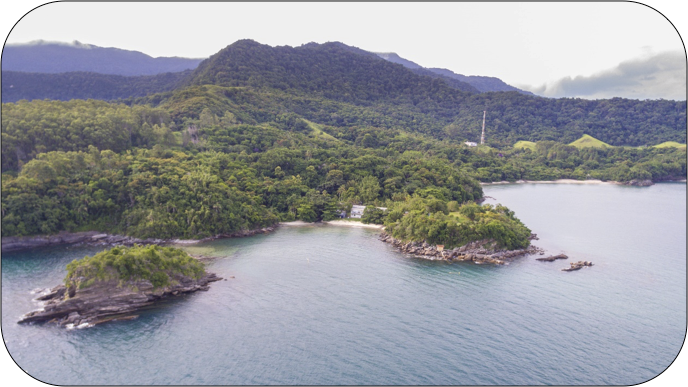
\includegraphics{figs/CEBIMar_pic.png}

\hypertarget{logistics}{%
\section{Logistics}\label{logistics}}

August 6-10, 2018 (+2 day for travel)

\hypertarget{venue-august-6-inpe}{%
\subsection{Venue, August 6: INPE}\label{venue-august-6-inpe}}

Opening of AmeriGEOSS Week Instituto Nacional de Pesquisas Espaciais
(INPE) São José dos Campos, São Paulo, Brasil

\hypertarget{venue-august-7-10-cebimar}{%
\subsection{Venue, August 7-10:
CEBIMar}\label{venue-august-7-10-cebimar}}

Centro de Biologia Marinha
(\href{http://cebimar.usp.br/index.php/en/}{CEBIMar}) - Universidade de
São Paulo Praia do Segredo - São Sebastião São Paulo, Brasil

\includegraphics{p2p-brazil-workshop_files/figure-latex/unnamed-chunk-2-1.pdf}

\hypertarget{organizers}{%
\section{Organizers}\label{organizers}}

\begin{itemize}
\tightlist
\item
  Pole-to-Pole Marine Biodiversity Observation Network (MBON) of the
  Americas - P2P MBON
\item
  Institute for Marine Remote Sensing (ImaRS), College of Marine
  Science, University of South Florida, St.~Petersburg, Florida, USA
\item
  Centro de Biologia Marinha (CEBIMar) \& Instituto de Biociências (IB)
  - Universidade de São Paulo, Brazil
\item
  AmeriGEOSS - Group on Earth Observations
\item
  Ocean Biogeographic Information System (OBIS)
\end{itemize}

\hypertarget{workshop-rationale}{%
\section{Workshop rationale}\label{workshop-rationale}}

This workshop is a first step for the implementation of the P2P network.
It addresses capacity building and science development for conservation
and management of living resources, to sustain critical ecosystem
services for communities in the region. The workshop participants will
develop standard protocols for field data collection, data formatting
and publishing, following international standards (e.g.~Darwin Core -
DwC). Efforts will also focus on data discovery and analysis using tools
provided by the Ocean Biogeographic Information System (OBIS) and the
GEO BON MBON. P2P incorporates the biodiversity priorities of various
GEO initiatives, including Blue Planet and AmeriGEOSS, and coordinates
with IOC/UNESCO (GOOS and OBIS), and other national and international
groups to serve the broadest possible community. This network will help
nations and regions to improve conservation planning and environmental
impact mitigation, serve the scientific community, and satisfy
commitments to the Intergovernmental Science-Policy Platform on
Biodiversity and Ecosystem Services (IPBES), Aichi Targets of the
Convention of Biological Diversity (CBD), and the UN 2030 Agenda for
Sustainable Development Goals (SDG's).

The P2P workshop:

\begin{itemize}
\tightlist
\item
  enhances coordination of data collection among nations;
\item
  improves the collection of harmonized data, developing data standards
  and methodologies for data management and dissemination without
  compromising national concerns;
\item
  integrates biodiversity information with physical and chemical data
  over time (status and trends); and
\item
  generates products needed for informed management of the ocean.
\end{itemize}

The workshop targets investigators and resource managers dedicated to
studying and conserving biodiversity of invertebrates in two important
coastal habitats: rocky shore intertidal zone and sandy beaches. This
activity targets participants from all nations in the Americas, from
pole to pole.

\hypertarget{instructors}{%
\section{Instructors}\label{instructors}}

\begin{itemize}
\tightlist
\item
  Eduardo Klein (OBIS) - Darwin Core (DwC) and OBIS tools
\item
  Ben Best (Ecoquants) - Data visualization and analysis tools using R
  software
\item
  Patricia Miloslavich (GOOS) - Protocols of the South American Research
  Group on Coastal Ecosystems (SARCE) and Essential Ocean/Biodiversity
  Variables (EOV/EBV) framework
\item
  Emmett Duffy (MarineGEO) - Predation and fouling community
  development, exotic invasions and biodiversity - an experimental
  approach.
\item
  Frank Muller-Karger (USF) - Satellite remote sensing
\item
  Maria Kavanaugh (OSU) - Satellite biogeography (seascape maps)
\item
  Maikon di Domenico (Universidade Federal do Paraná) - sandy beaches*
\item
  Pete Raimondi (UCSC -- PISCO / MARINe)\emph{ (}waiting for
  confirmation)
\end{itemize}

\hypertarget{required-workshop-materials}{%
\section{Required workshop
materials}\label{required-workshop-materials}}

\begin{itemize}
\item
  Participants must bring a laptop computer with the following programes
  installed (with latest version, as of 2018-03-20):

  \begin{itemize}
  \tightlist
  \item
    \href{https://cran.r-project.org}{R} (3.4.4)
  \item
    \href{https://www.rstudio.com/products/rstudio/download/\#download}{RStudio}
    (1.1.442)
  \item
    \href{https://git-scm.com/downloads}{Git} (2.16.2)
  \end{itemize}

  These are available for Windows, Mac or Linux operating systems.
\item
  Install additional packages by running the following line of code in
  your R terminal:

\begin{Shaded}
\begin{Highlighting}[]
\KeywordTok{source}\NormalTok{(}\StringTok{"https://github.com/marinebon/p2p-brazil-workshop/master/scripts/install-R-packages.R"}\NormalTok{)}
\end{Highlighting}
\end{Shaded}
\item
  Github.com/io, for code / R-generated examples / landing page:

  \begin{itemize}
  \tightlist
  \item
    ioos.github.io/BioData-Training-Workshop: IOOS template
  \item
    ohi-science.org/data-science-training: bookdown OHI
  \item
    marinebon.github.io/p2p-brazil-workshop: bookdown min example.
    Bookdown renders Rmarkdown into easy to navigate book format.
  \end{itemize}
\item
  SARCE sampling protocols. The past experience could be replicated (and
  it will be desirable if we want to make comparison in time) see the
  SARCE site and it protocols. The SARCE data will be in OBIS after the
  next harvest.
\item
  Full snorkeling gear
\end{itemize}

\hypertarget{preliminary-agenda}{%
\section{Preliminary Agenda}\label{preliminary-agenda}}

\label{tab:unnamed-chunk-3}Agenda (draft)

Time

Description

Aug 6, day 1, Mon: AmeriGEOSS Week (INPE; São José dos Campos)

9 am - noon

Opening of AmeriGEOSS Week at the Instituto Nacional de Pesquisas
Espaciais (INPE; São José dos Campos) {[}Gutierrez, Montes{]}

2 pm

Departure to the Centro de Biologia Marinha (CEBIMar) in São Sebastião

4 pm

Arrival at CEBIMar (lodging TBD)

7 pm

Group dinner (TBD)

Aug 7, day 2, Tue: Field sampling of intertidal rocky shore
invertebrates

7:30 - 8:30 am

Breakfast (it'd be good have it at CEBIMar)

8:30 - 9 am

Welcome and workshop briefing {[}Montes{]}

9 - 9:45 am

Rocky Intertidal sampling protocol \& taxonomy of invertebrates
{[}Miloslavich{]}

9:45 - 10 am

Cross-referencing Essential Ocean Variables and Essential Biodiversity
Variables frameworks

10 - noon

Field sampling activity (TBD) {[}Marques{]}

12:30 - 2 pm

Lunch

Aug 7 afternoon: back at CEBIMar

2 - 2:30 pm

How to register data collected in the field. {[}Klein, Montes{]}

2:30 - 3:15 pm

Intro to Reproducible Research Tools: R, Rmarkdown, Github {[}Best{]}

3:15 - 5 pm

Open computer lab work

7 pm

Group dinner (TBD)

Aug 8, day 3, Wed: Field sampling of sandy beaches invertebrates

7:30 - 8:30 am

Breakfast

8:45 - 9 am

Workshop briefing: Day 3 {[}Montes{]}

9 am - 10 am

Sandy beaches sampling protocol \& taxonomy for invertebrates {[}TBD{]}

10 am - noon

Field sampling activity (TBD) {[}Marques{]}

12:30 - 2 pm

Lunch

Aug 7 afternoon: back at CEBIMar

2 pm - 2:30 pm

How to register data collected in the field. {[}Klein{]}

2:30 - 3:15 pm

From data to plots to websites {[}Best{]}

3:15 - 5 pm

Open computer lab work

5 - 6 pm

MarineGEO, Predation and fouling community development, exotic invasions
and biodiversity - an experimental approach {[}Duffy{]}

7 pm

Group dinner (TBD)

Aug 9, day 4, Thu: OBIS

7:30 - 8:30 am

Breakfast

8:45 - 9 am

Workshop briefing: Day 4 {[}Montes{]}

9:00 - 9:30 am

Ocean Biogeographic Information System (OBIS) for data sharing, analysis
and discovery. {[}Klein{]}

9:30 - 10:30 am

International data standards: Darwin Core (DwC), QA/QC, publishing to
OBIS w/ IPT {[}Klein{]}

10:30 - 10:45 am

Break

10:45 - 11:30 am

Use of taxonomy databases (e.g.~WoRMS) {[}Klein{]}, Practical exercises
{[}Best{]}

11:30 - noon

SARCE Case Study {[}Klein, Miloslavich{]}

12:00 - 1:30 pm

Lunch

1:30 - 2:00 pm

The MBON Ocean Explorer: an integrated visualization of OBIS records and
satellite data {[}Muller-Karger, Best{]}

2:00 - 5:00 pm

Data cataloging using WoRMS, data formatting using DwC
{[}Participants{]}

7 pm

Group dinner

Aug 10, day 5, Fri: Data analysis \& viz

7:30 - 8:30 am

Breakfast

8:45 - 9 am

Workshop briefing: Day 5 {[}Montes{]}

9 - 9:30 am

Data visualization and analysis tools using R software {[}Best{]}

9:30 - 10 am

Satellite biogeography and dynamic seascape maps as tools for scaling in
situ biodiversity observations {[}Montes{]}

10 - 10:15 am

Break

10:15 - noon

Pushing data into OBIS {[}Participants{]}

noon - 1:30 pm

Lunch

1:30 - 3 pm

Pushing data into OBIS {[}Participants{]}

3 pm

Adjourn

\hypertarget{survey}{%
\section{Survey}\label{survey}}

Loading\ldots{}

\hypertarget{resources}{%
\section{Resources}\label{resources}}

\begin{itemize}
\tightlist
\item
  \href{http://www.iobis.org/manual/}{Ocean Biogeographic Information
  System (OBIS) - Manual}
\item
  \href{http://r4ds.had.co.nz/}{R for Data Science}
\item
  \href{http://rspatial.org}{Spatial Data Analysis and Modeling with R}
\item
  \citep{hijmans_species_2017}
\end{itemize}

\bibliography{style/zotero\_mbon-p2p.bib,style/packages.bib}


\end{document}
